\documentclass[11pt]{article}

\usepackage[margin=1in]{geometry}
\usepackage{amsmath}
\usepackage{xurl}
\usepackage{hyperref}
\usepackage{graphicx}
\usepackage{subcaption}
\usepackage{float}
\usepackage{array}

\title{Developing a Head-to-Head Prediction Model for International Soccer Matches}
\author{Somak Shivlani, Javier Carillo}
\date{\today}

\newcommand{\codepath}[1]{\nolinkurl{#1}}

\begin{document}

\maketitle

\section{Introduction}

Soccer (or football, as it is known outside North America) is the most followed sport globally, with billions of fans tuning into the FIFA World Cup every four years. Beyond its massive cultural impact, soccer is a highly profitable industry, generating an estimated \$30 billion worldwide annually.

Predicting match outcomes and team performance has emerged as a crucial topic and a compelling challenge in sports analytics. These predictive models have wide-ranging applications, including tournament forecasting, statistical modeling, performance evaluation, team seeding, valuation, strategy formulation, and player recruitment.

Furthermore, sports betting represents another high-value market heavily reliant on these analytics to establish betting lines and calculate payouts. With an estimated market cap of \$100 billion USD in soccer alone, accurate outcome prediction can be highly lucrative. However, soccer remains an inherently complex sport, influenced by numerous dynamic variables and exhibiting a high degree of variance.

The long-term objective of this project is to develop a\textbf{ head-to-head prediction model} capable of estimating the likely outcome between two international teams. Such a model can be utilized to simulate tournament brackets, evaluate relative team strength, and forecast match results beyond traditional ranking systems.

We focus our predictions specifically on the international teams participating in the 2026 FIFA World Cup. The project combines international match history, Elo ratings, and player-level expected-goals statistics from Europe's top five leagues to create head-to-head national-team features. These features are then evaluated through both interpretable baseline models and non-linear ensemble models. The final repository therefore contains two connected modeling tracks: a baseline multiclass outcome track using Logistic Regression and SVM, and an xG-centered tournament simulation track using Random Forest, XGBoost, and a score-based expected-points model.

Of particular importance to our methodology is a metric widely utilized in modern soccer analytics: \textbf{Expected Goals (xG)}. This statistic quantifies the quality of goal-scoring opportunities, estimating the number of goals a player or team should realistically score in a specific matchup based on established predictive models. In our study, we will utilize the xG data provided by the Understat database to compare against actual team performance and evaluate our custom variables. xG is calculated by assigning a probability (ranging from 0 to 1) to every shot taken, based on historical data from thousands of similar attempts. The models determine this probability by analyzing variables such as the shot's distance and angle to the goal, the body part used (e.g., foot vs. header), the type of play (e.g., open play, corner kick, penalty), and the preceding action (e.g., a through ball or a cross).


This framework aims to predict the outcome of these matchups, estimate group-stage expected points, and simulate possible knockout paths. Our research is guided by the following questions:
\begin{itemize}
\item To what extent do individual player statistics from the top 5 European leagues influence the probability of their respective national teams winning an international matchup?

\item How effectively does the past five years of international head-to-head history predict future tournament outcomes when combined with recent club-level player data?

\item How accurately can a logistic regression model predict the specific match outcome (win or draw) of a 2026 World Cup fixture using this combined dataset?

\item How do non-linear ensemble models, specifically Random Forest and XGBoost, perform when trained on engineered xG-based national-team features?

\item Can a score-based model estimate expected points in the group stage, where draws are possible and should not be forced into a binary winner prediction?

\item Can model outputs be used to simulate the 2026 World Cup knockout bracket and estimate the sensitivity of the projected champion to model choice?

\end{itemize}

\section{State of the Art}

The existing literature on this topic is extensive, spanning multiple years and encompassing methodologies that range from traditional statistics to sophisticated deep learning algorithms. Recent research underscores the predictive power of underlying performance metrics within domestic competitions, directly informing our variable selection. A 2025 study by Bat-Erdene and Peloguin \cite{2025europeData} analyzed team success across Europe's top five leagues during the 2023-24 and 2024-25 seasons. Through regression analysis, the authors determined that expected goal difference (xGD) and chance creation metrics, specifically expected goals plus expected assists per 90 minutes (xG+xAG/90), are among the strongest predictors of a team's points per match. Their models also demonstrated that defensive solidity, measured by lower expected goals against (xGA), is equally crucial for distinguishing elite teams from average competitors. This research validates our approach by confirming that advanced expected metrics from major European leagues serve as robust, standardized indicators of player and squad quality. We will aggregate these metrics to forecast international tournament success.

A foundational work in sports outcome prediction is the 2020 comprehensive review by Horvat and Job \cite{2020mlreview}, which evaluates the primary machine learning methods utilized in this domain. The authors analyzed 39 papers published between 1996 and 2020 across five major team sports: basketball, soccer, American football, baseball, and cricket. Their review indicates that neural networks are historically the most widely adopted machine learning models for predicting sports outcomes, although Support Vector Machines, Naïve Bayes, and logistic regression are also highly prevalent. For soccer specifically, prediction accuracies generally range between 54\% and 93\%, with artificial neural networks, logistic regression, and random forests frequently applied to major European leagues. Horvat and Job emphasize that rigorous feature selection and extraction are critical preliminary steps that significantly enhance both the efficiency and performance of these algorithms. Ultimately, they conclude that soccer is uniquely challenging to predict compared to higher-scoring sports like basketball. This difficulty stems from its low-scoring nature and the high mathematical probability of draws, highlighting the necessity for models that can effectively handle high variance and multiclass outcomes.

Classical football forecasting research has also relied heavily on score models and team-rating systems. Dixon and Coles \cite{dixoncoles1997} introduced an influential statistical model for association-football scores using goal-count distributions and betting-market evaluation. This motivates our score-based group-stage model, since World Cup group matches can end in draws and should not always be reduced to a forced winner. Another common way to summarize team strength is the Elo rating system, originally developed by Elo for chess ratings \cite{elo1978}. Elo updates a team's rating after each match based on the difference between the observed result and the result expected from the two teams' pre-match ratings. In football analytics, Hvattum and Arntzen \cite{hvattum2010elo} showed how Elo-style ratings can be used as inputs for match-result prediction, while Constantinou and Fenton \cite{constantinou2013piratings} proposed football-specific dynamic ratings that similarly encode changing team strength over time. These works justify the use of Elo as a baseline historical-strength variable in our partner Logistic Regression and SVM models.

Finally, to bridge the gap between historical methods and modern data availability, a recent overview by Bunker, Yeung, and Fujii \cite{bunker2024machinelearningsoccermatch} provides clear direction for current sports analytics research. Their analysis reveals that while gradient-boosted tree models, such as CatBoost, achieve state-of-the-art performance on simple datasets containing only basic match goals, there is a critical need to evaluate predictive models on richer datasets that incorporate detailed player and team-level statistics. By utilizing comprehensive five-year player performance data from Europe's top five leagues, our project directly answers this call for event-driven feature engineering. Additionally, the authors strongly emphasize that predictive models must remain highly interpretable to be practically useful for team management, coaches, and performance analysts. This requirement underscores our methodological choice of logistic regression for the interpretable baseline. At the same time, the same literature motivates the inclusion of Random Forest and XGBoost as non-linear ensemble methods, since tree-based models can capture threshold effects and feature interactions that may be missed by a purely linear classifier.

\section{Materials and Methods}

\subsection{Datasets}

To support the development of the head-to-head prediction model for the 2026 FIFA World Cup, data was aggregated from several primary sources and filtered to ensure tournament relevance:
\begin{itemize}

\item International match results were extracted using the \texttt{worldfootballR} package \cite{zivkovic_worldfootballR}, which interfaces with comprehensive football statistics databases. These records were used to build the combined historical match table used by the score model and the final full-history evaluation.

\item Additional recent head-to-head World Cup-team match history from 2018 through 2026 was compiled from Transfermarkt-style national-team game data. This supplied more recent tournament-relevant match results and metadata such as competition, round, goals, stadium, attendance, and neutral-site information.

\item To quantify baseline team strength in the partner baseline track, historical international team Elo ratings were integrated via Kaggle datasets \cite{alnimri_elo_ratings}. Elo ratings summarize national-team strength from past match outcomes and were used as matchup-difference variables, such as \texttt{diff\_elo}, in the Logistic Regression and SVM workflows.

\item At the individual level, player performance metrics including expected goals (xG), non-penalty xG, expected assists (xA), shots, key passes, xG chain, and xG buildup were scraped and merged from Understat player data, capturing data across the Top 5 European leagues from the 2021--2022 season up through March 31, 2026 \cite{fbref_top5_data}. 

\item This was supplemented with comprehensive player profile data updated to 2026, sourced from a secondary Transfermarkt Kaggle dataset \cite{cariboo_transfermarkt}. 

\item Official 2026 World Cup schedule and bracket information was stored as structured tournament inputs. The repository includes the official schedule PDF along with group assignments, seed paths, and bracket slot mapping tables.

\end{itemize}
To align the dataset exclusively with the scope of the upcoming tournament, the compiled records were filtered to retain only the national teams that have officially qualified for the 2026 World Cup, alongside the active players representing those specific nations.

For the final repository, curated project data is organized under \codepath{data}. The file \codepath{MatchData.csv} is retained for the baseline Logistic Regression and SVM workflows, with a copy in \codepath{data/legacy_svm}. The ensemble-model inputs are stored under \codepath{data/processed}. The player-feature table \codepath{understat_tm_merged_specific_nation_filtered.csv} contains the merged xG and player-profile data after filtering to World Cup nations. From this file, two derived national-team feature tables were generated: \codepath{team_season_features.csv}, which preserves season-level team summaries, and \codepath{team_current_features.csv}, which uses a recency-weighted aggregation to represent current national-team form. The match-history files include \codepath{national_team_games_h2h_wc_teams_2018_2026.csv} for recent head-to-head results and \codepath{historical_matches_combined_1672.csv}, a combined full-history dataset of 1,672 match rows used for the final 80/20 evaluation. Tournament inputs are stored under \codepath{data/processed/tournament}, while final model metrics, expected-points outputs, confusion matrices, and simulation summaries are stored under \codepath{data/results}.

\subsection{Repository Implementation}

The repository is organized to separate documentation, data, and executable source code. The \codepath{docs} folder contains the presentation and this final report. The \codepath{data} folder contains only curated project inputs and outputs needed to reproduce or explain the final results. Large raw source dumps are intentionally excluded, while processed model-ready CSV files are included.

Source code is stored under \codepath{src}. The baseline partner workflows are kept in \codepath{src/lr_model.r}, \codepath{src/svm_model.r}, and \codepath{src/data_processing}. Notebook-based exploratory scraping, merging, and visualization work is stored in \codepath{src/notebooks}. Python utilities in \codepath{src/python} were used to scrape and merge Understat, Transfermarkt, and country-mapping data. The current World Cup modeling pipeline is stored in \codepath{src/r}. In that folder, \codepath{wc2026_head_to_head_models.R} creates the xG-based national-team features and trains Random Forest and XGBoost; \codepath{wc2026_group_stage_expected_points.R} creates score-based group-stage expected-points outputs; \codepath{wc2026_hybrid_knockout_comparison.R} combines the score model with the winner models for full tournament simulations; \codepath{wc2026_schedule_map.R} and \codepath{wc2026_bracket_simulation.R} structure the 2026 schedule and bracket; and \codepath{wc2026_result_slide_assets.R} generates slide-ready confusion matrices and tree-model assets.

\subsection{Data Integration and Cleaning}

To prepare the raw datasets for machine learning applications, a comprehensive data manipulation pipeline was implemented using the \texttt{tidyverse} framework in R. The following subsections detail the methodology for merging disparate data sources, engineering team-level features, and preparing the final dataset for model training.

\subsubsection{Rolling Joins and Nested Data Structures}
\label{subsec:rolling_joins}
A primary challenge involved unifying daily match data with periodic Elo ratings and static player statistics. To prevent future information from leaking into historical matches, rolling joins were utilized (specifically, \texttt{join\_by(Home == team, closest(Date >= date))}) to ensure each match was associated with the most up-to-date Elo rating strictly prior to kickoff. For player statistics, individual records were nested by nation, effectively compressing the entire roster into a single dataframe entity. This facilitated a cleaner join process, attaching a complete roster profile to both the Home and Away sides of the match ledger.

\subsubsection{Team Name Standardization and Match Formatting}
\label{subsec:name_standardization}
Because the project combines data from Understat, Transfermarkt, worldfootballR, Kaggle, and manually structured tournament files, country names had to be standardized before merging. A country mapping file was used to align variants such as alternate spellings, punctuation differences, and federation naming conventions. Match data was also reshaped into a consistent two-team format with fields for \texttt{team}, \texttt{opponent}, \texttt{team\_goals}, \texttt{opponent\_goals}, \texttt{match\_date}, competition, round, neutral-site status, and source. For Transfermarkt-style files where scores are represented as an aggregate string, the aggregate was parsed into home goals and away goals before being converted into team-opponent rows.

\subsubsection{Elo Integration}
\label{subsec:elo_integration}
Elo ratings were used as a compact summary of historical national-team strength in the baseline modeling branch. The Elo system assigns each team a rating and updates it after each match according to whether the team performed better or worse than expected from the rating gap \cite{elo1978,hvattum2010elo}. The feature is useful because it captures information not directly represented by player xG data, such as prior international results, team-level consistency, and strength of schedule. After joining each match to the most recent available pre-match Elo rating for both sides, the model used rating differences rather than raw ratings. This produced a direct head-to-head variable, \texttt{diff\_elo}, where a positive value indicates that the home or row team had a higher rating than its opponent at the time of the match.

\subsubsection{Symmetrical Data Augmentation}
\label{subsec:augmentation}
For international tournaments played at neutral venues, standard ``Home'' and ``Away'' designations are administrative and risk introducing positional bias into the model. To neutralize this, symmetrical data augmentation was applied. A secondary dataset was generated where every ``Home'' variable was explicitly inverted to ``Away'' and vice versa, encompassing goals, Elo ratings, and player statistics. By concatenating the original and swapped datasets, the sample size was effectively doubled. This forces the model to recognize that Team A playing Team B is mathematically identical to Team B playing Team A, represented by inverted signs on the differential features.

\subsubsection{Feature Engineering: Roster Aggregation}
\label{subsec:roster_aggregation}
Because the prediction target is team-level match outcomes, individual player statistics were aggregated into national squad features. A custom function was developed to filter the nested player data by total minutes played, isolating the top eleven players to represent the core squad. Features were processed based on their statistical nature:
\begin{itemize}
    \item \textbf{Counting Statistics:} Metrics such as total goals, expected goals (xG), and market value were summed.
    \item \textbf{Rate Statistics:} Metrics such as xG per 90 minutes (\texttt{xg\_per90}) and player height were averaged.
    \item \textbf{Imputation Scaling:} To account for instances of incomplete scraped data, a proportional scaling factor ($11 / n$) was applied to project partial squad data up to a full eleven-man equivalent.
\end{itemize}

\subsubsection{Differential Feature Construction}
\label{subsec:differential_features}
Rather than supplying the model with absolute statistical totals, the data was condensed into differential head-to-head variables. By subtracting the Away team's aggregate statistics from the Home team's aggregate statistics (e.g., \texttt{diff\_total\_xg}), the feature space directly represents the quantitative gap in quality between the two sides. This dimensional reduction is computationally efficient and enhances the interpretability of feature importance metrics.

\subsubsection{xG-Based National-Team Feature Pipeline}
\label{subsec:xg_pipeline}
In addition to the top-eleven aggregation used in the baseline models, a second feature-engineering pipeline was built to represent national teams through broader squad-level xG profiles. Player rows were grouped by nation and season, then collapsed into totals, per-90 rates, depth measures, and concentration measures. Important features included total xG, non-penalty xG, xA, shots, key passes, xG chain, xG buildup, market value, international caps, and age-related summaries. Rate features such as \texttt{xg\_per90}, \texttt{np\_xg\_per90}, \texttt{xa\_per90}, \texttt{shots\_per90}, and \texttt{key\_passes\_per90} were computed from national-team player totals.

The passing and chance-creation variables come from the Understat-style player tables \cite{understat}. In this context, \textbf{xA} is expected assists: the expected-goal value of shots that a player assisted. \textbf{Key passes} are passes that directly lead to a shot. \textbf{xGChain} assigns a player credit for the xG value of possessions in which the player was involved, so it captures broader attacking participation rather than only shots or final passes. \textbf{xGBuildup} is similar but excludes the final shot and assisted-shot actions, making it a proxy for deeper buildup contribution. These variables were included because international teams with stronger creators and buildup players may generate higher-quality chances even when the final goal count is noisy.

To avoid relying only on raw attacking totals, additional squad-depth features were engineered. These included top-one, top-three, and top-five xG totals and shares, Herfindahl-style xG concentration metrics, counts of players above minute and xG thresholds, and position-bucket minute shares for goalkeeper, defender, midfield, and attack roles. Current-form team features were then produced using a recency-weighted average across seasons, allowing newer player performance to matter more than older seasons while still preserving information from the full five-year window.

For model training, each match row was joined twice against the national-team feature table: once for the team and once for the opponent. For every numeric feature, three matchup variables were produced: the team-opponent difference, the sum of the two teams, and the absolute difference. This created a head-to-head representation that allowed the model to learn both relative strength and matchup balance.

\subsection{Descriptive Feature Analysis}

To address the structure of the engineered dataset before modeling, we examined the recency-weighted current national-team feature table. This table contains 47 national teams and 89 engineered columns, including attacking production, chance creation, squad depth, player concentration, market value, caps, age, and position-share variables. Because many features are measured on different scales, the exploratory analysis focuses on correlations and standardized distributions rather than raw magnitudes alone.

Figure \ref{fig:feature_correlation_heatmap} shows the correlation matrix for the main engineered variables. The attacking volume variables, including total xG, non-penalty xG, xA, shots, key passes, and xGChain, are strongly positively correlated. This is expected because teams with more high-minute attacking players in top European leagues tend to accumulate more shots, final passes, and possession involvement. Market value and caps also correlate with several production features, suggesting that player valuation and international experience partly track squad quality. However, concentration and depth variables capture different information: a high xG concentration means a team relies heavily on a small number of attackers, while the player-count and attack-depth variables measure how much production is distributed across the squad.

\begin{figure}[H]
     \centering
     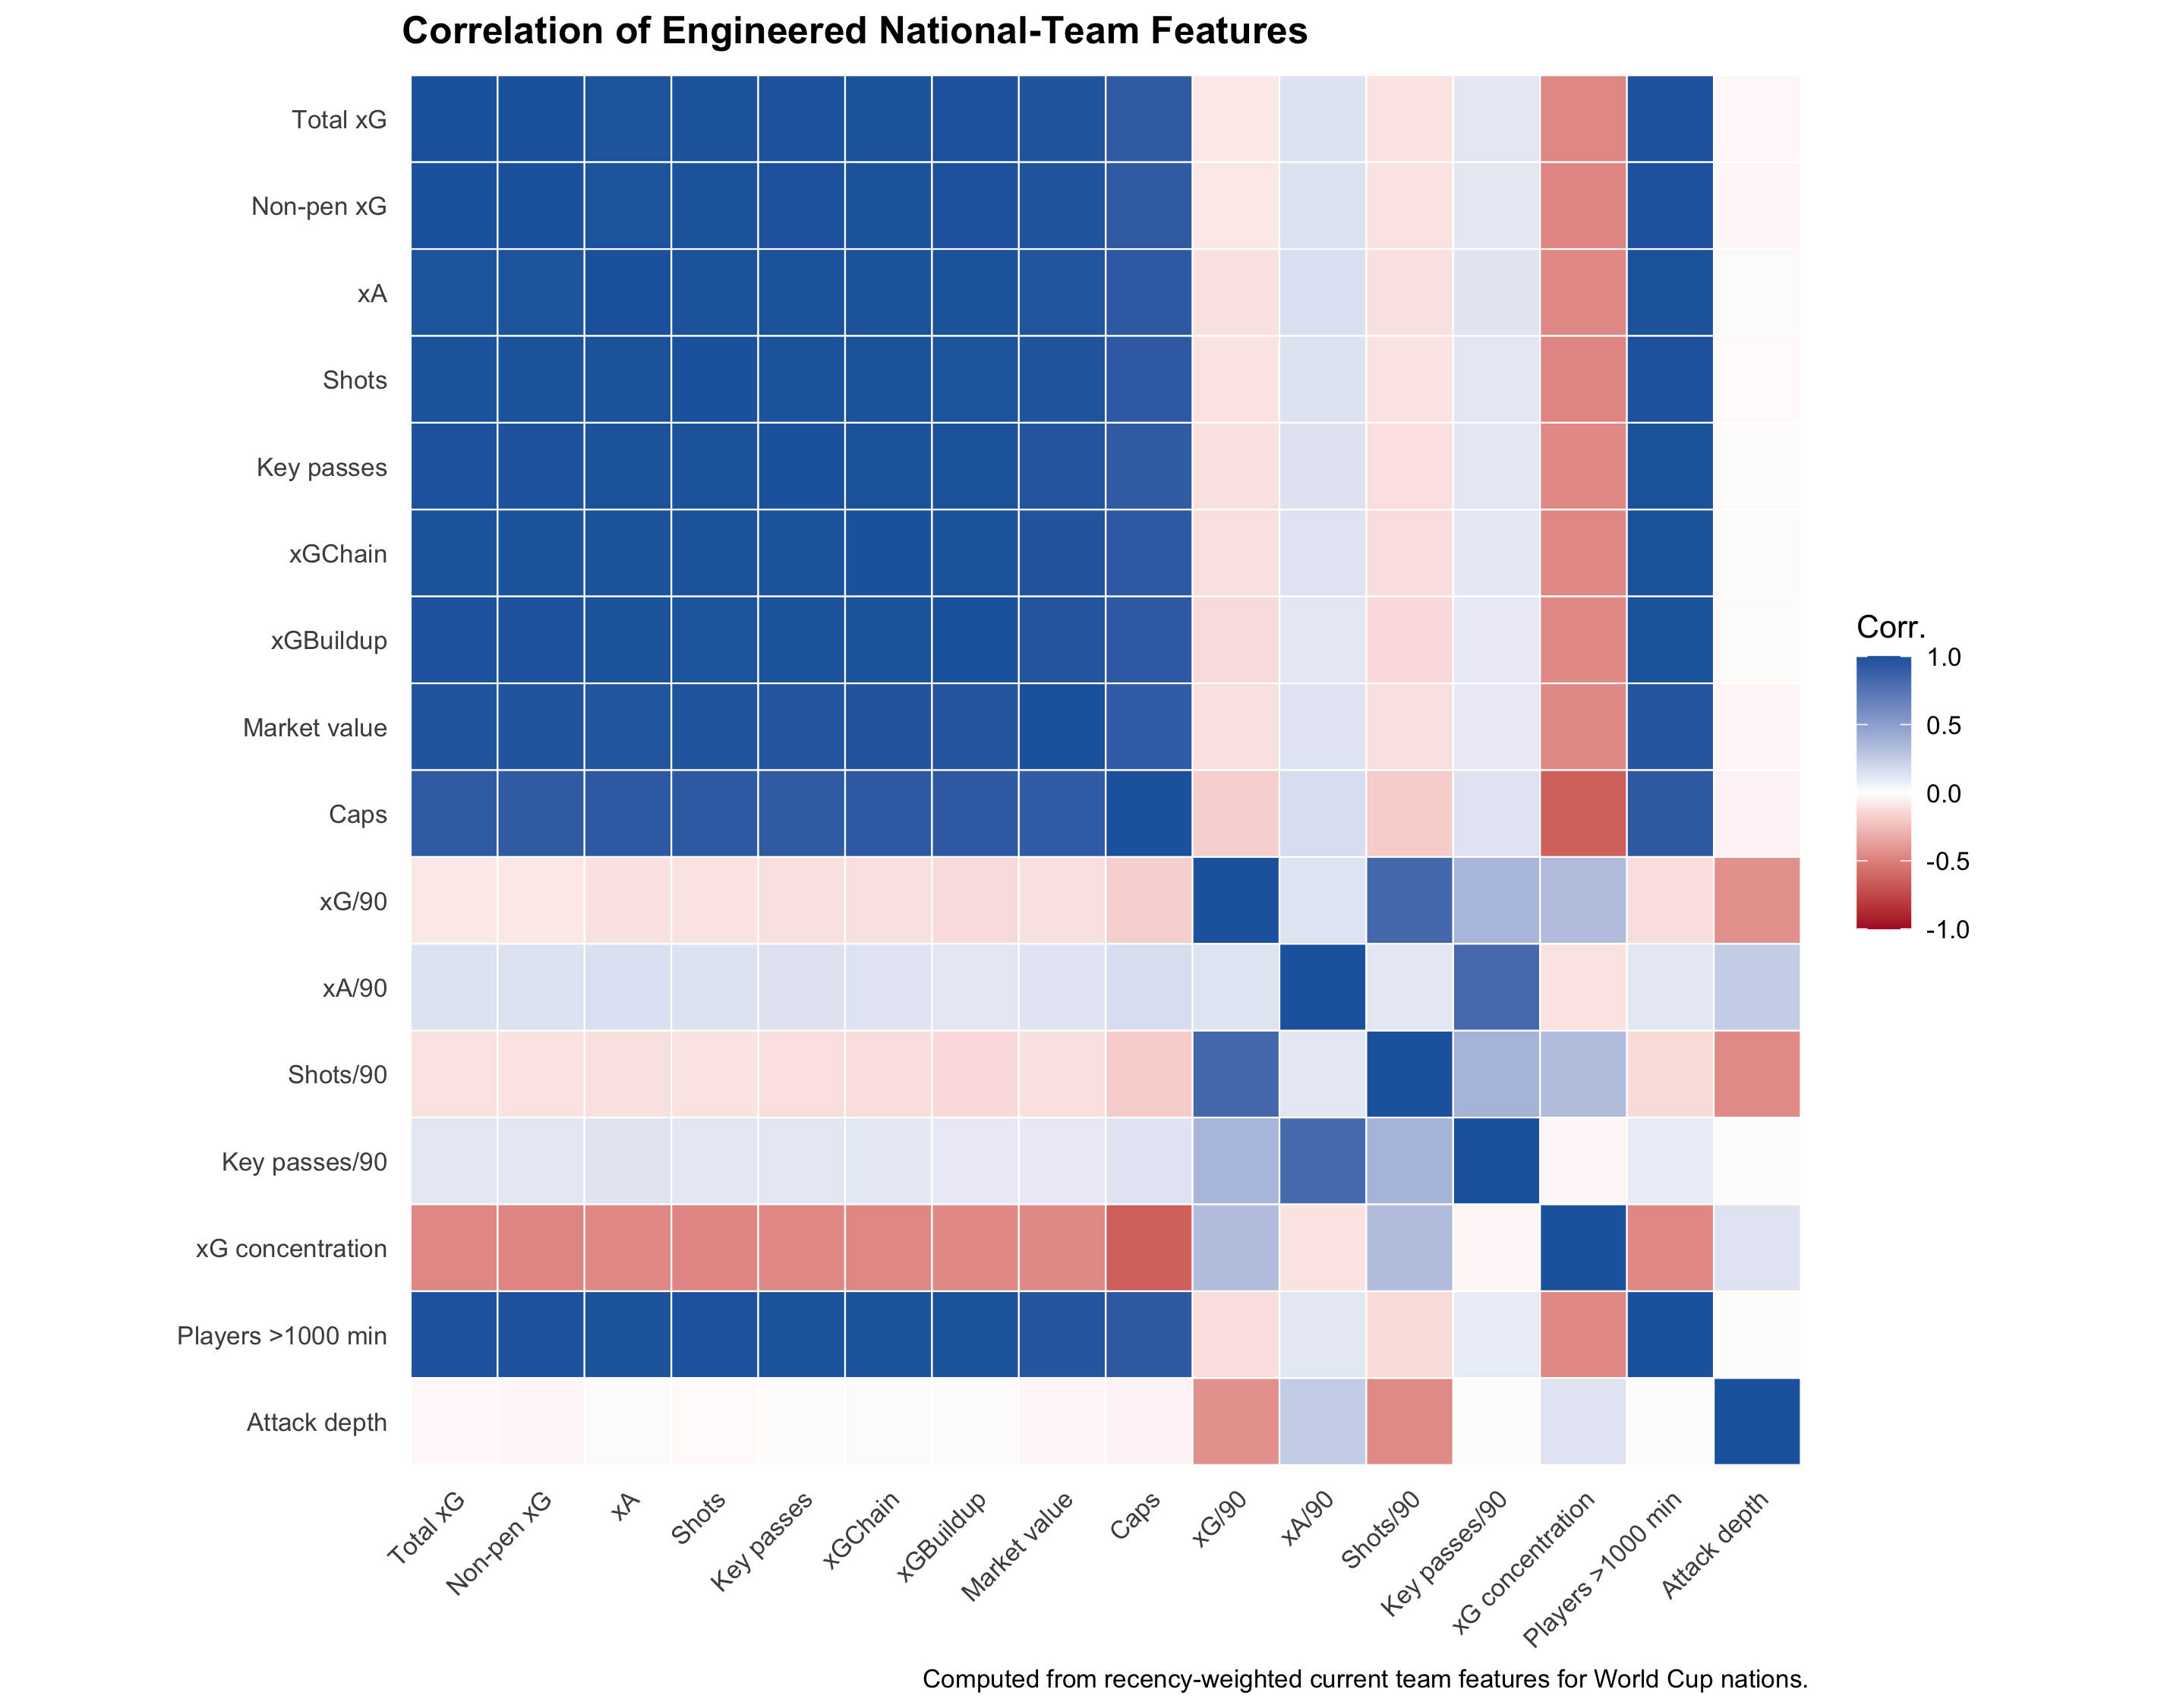
\includegraphics[width=0.92\textwidth]{feature_correlation_heatmap.png}
     \caption{Correlation heatmap of selected engineered national-team features. The plot shows that many attacking and chance-creation variables are related, while concentration and depth features provide separate information about squad structure.}
     \label{fig:feature_correlation_heatmap}
\end{figure}

Figure \ref{fig:feature_distribution_boxplots} shows standardized boxplots for selected engineered variables. The distributions are not symmetric: market value, xG totals, xA totals, and xGChain are right-skewed because a small number of countries have many elite players in high-value European clubs. This skewness supports using tree-based models in addition to linear models, since Random Forest and XGBoost can model thresholds and interactions without assuming that each feature has a linear effect. The boxplots also show why scaling was required for the baseline Logistic Regression and SVM workflows.

\begin{figure}[H]
     \centering
     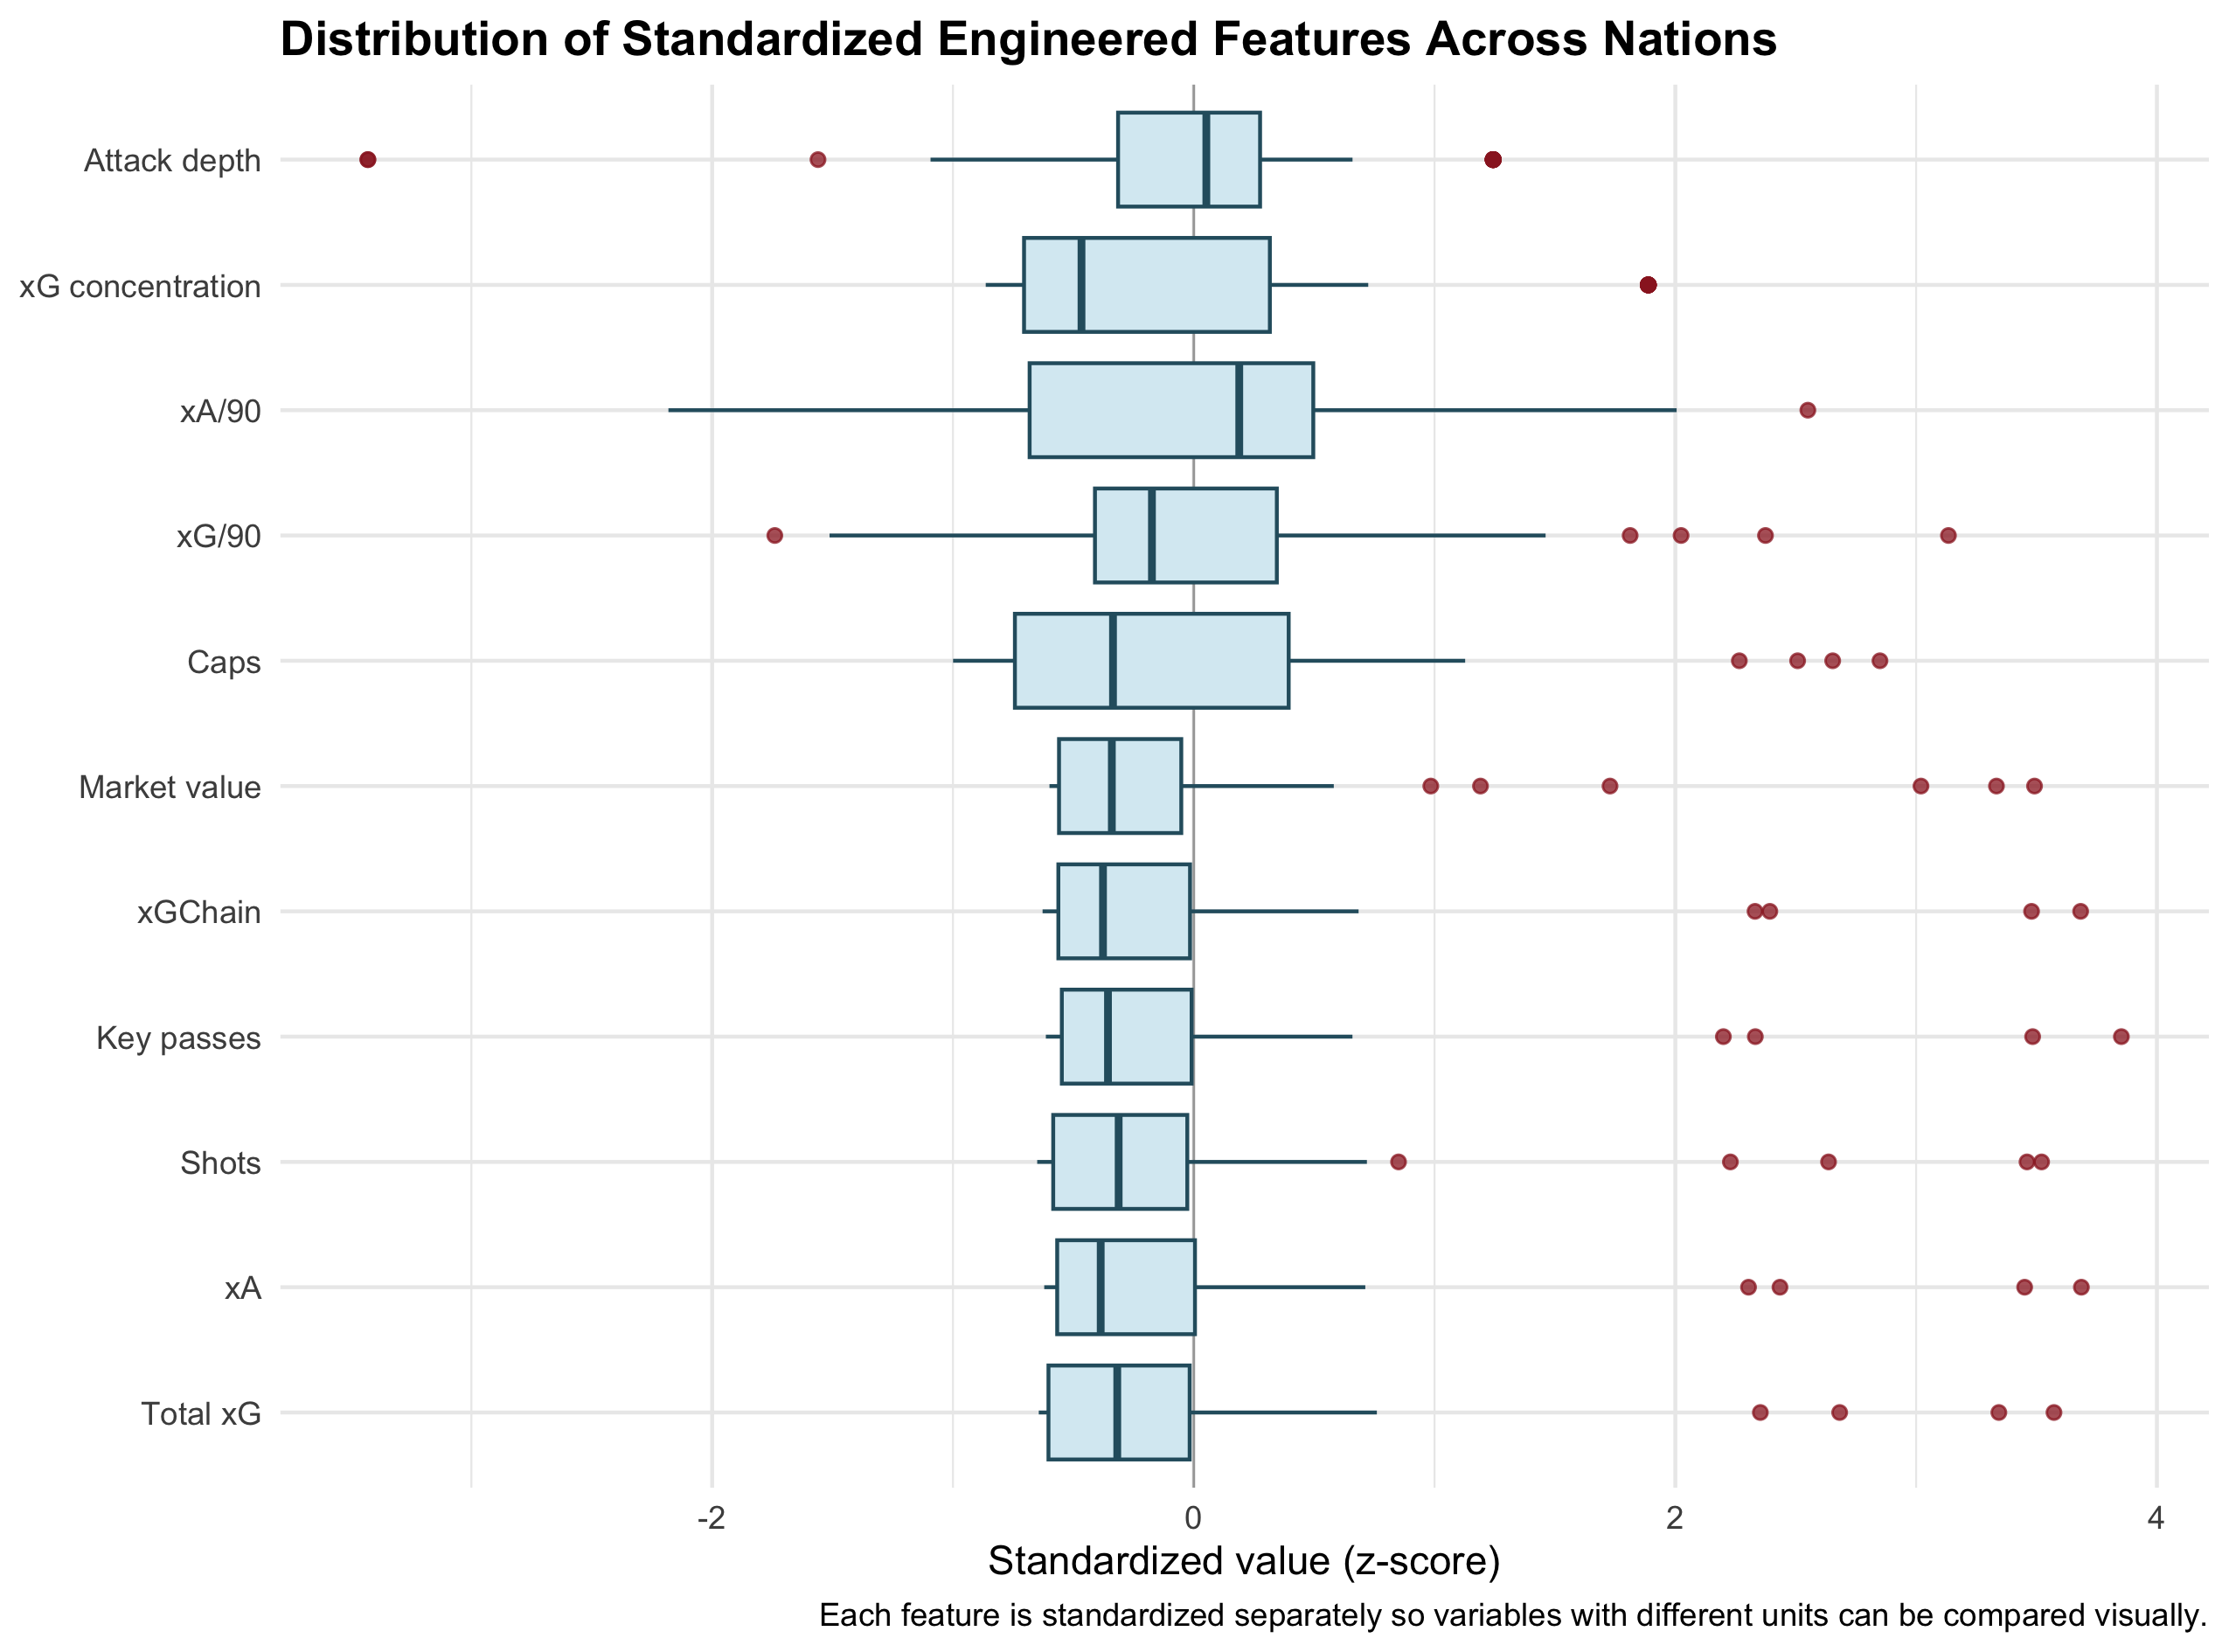
\includegraphics[width=0.88\textwidth]{feature_distribution_boxplots.png}
     \caption{Standardized boxplots for selected engineered features across World Cup nations. Each variable is converted to a z-score before plotting so that features with different units can be compared.}
     \label{fig:feature_distribution_boxplots}
\end{figure}


\subsection{Methods}

A diverse suite of four machine learning models was evaluated: Multiclass Logistic Regression, Linear Support Vector Machines (SVM), Random Forest, and XGBoost. Because international football match results exhibit inherent class imbalance, class weights were applied in the baseline multiclass models to penalize misclassifications of minority outcomes and prevent predictive bias.

The Random Forest and XGBoost branch was implemented in R using the \texttt{tidymodels} framework. Unlike the multiclass Logistic Regression and SVM baselines, these models were trained as binary head-to-head classifiers, where each row represents a team-opponent matchup and the target is whether the team wins. Drawn matches are treated as non-wins in this binary setup. The Random Forest model used 1,000 trees, a square-root style rule for \texttt{mtry}, and a minimum node size of 5. The XGBoost model used 1,000 trees, depth 4, a learning rate of 0.05, \texttt{mtry} set to approximately 70\% of the predictor count, and a minimum node size of 5. These tree-based models were selected because they can capture non-linear interactions between squad quality, xG production, player concentration, and opponent strength.

\subsubsection{Score-Based Expected Points Model}
\label{subsec:score_model}
Because group-stage football allows draws, a separate score-based model was developed instead of forcing every group match to have a binary winner. This model estimates each team's expected goals in a fixture using a Poisson generalized linear model. The model is trained on historical match scorelines and produces an expected goal rate for each side. From those rates, match scorelines are simulated, group-stage points are assigned using the standard FIFA rules of three points for a win, one point for a draw, and zero points for a loss, and the process is repeated to estimate expected points, expected goal difference, qualification probabilities, group-win probability, and third-place probability.

This score model serves two purposes. First, it provides a more realistic group-stage table because teams can draw. Second, it supplies scoreline mechanics for the tournament simulation, including expected goals, extra-time handling, and penalty resolution when knockout matches remain tied. The score model is reported separately from the Random Forest and XGBoost winner models because it solves a different prediction task: estimating scores and group points rather than directly classifying which side wins.

\subsubsection{Hybrid Knockout Simulation}
\label{subsec:hybrid_simulation}
For tournament interpretation, the trained tree models were connected to a bracket simulation workflow. The official 2026 World Cup schedule and bracket slots were mapped into structured CSV files, projected group finishers were assigned to knockout slots, and the model outputs were used to simulate the bracket. The final hybrid workflow combines the score model with each winner model. The score model handles group-stage expected points and scoreline-based match mechanics, while Random Forest or XGBoost supplies head-to-head win probabilities for knockout advancement. A separate score-only version is also retained as a baseline to show how tournament results change when advancement is driven only by the score model.

Monte Carlo simulation was used because a tournament forecast should represent uncertainty rather than only one deterministic bracket. For each model, the tournament was sampled 200 times. Each run samples match outcomes from the model probabilities, advances teams through the bracket, and records the champion. The resulting champion probabilities therefore represent the frequency with which a team wins the simulated tournament under that model's assumptions.

\subsection{Evaluation}

To accurately simulate real-world predictive performance, the dataset was partitioned chronologically rather than randomly. The data was ordered by date, allocating the earliest 80\% of matches to the training set and the most recent 20\% to the testing set. For the full-history tree-based branch, this produced a 1,672-row dataset with 335 matches in the held-out test set. The held-out test period spans from June 10, 2022 through January 18, 2026.

Furthermore, to satisfy the mathematical requirements of scale-sensitive algorithms, all differential numerical features were centered and scaled. Crucially, the scaling parameters (mean and standard deviation) were derived strictly from the training data using the \texttt{caret} package. These identical parameters were subsequently applied to the testing data, ensuring zero data leakage between the historical training phase and the evaluation phase.

To optimize the parametric models and prevent overfitting, cross-validation (CV) was utilized extensively during the training phase. Specifically, CV was paired with Lasso ($L_1$) regularization to isolate the most significant predictive variables and derive a compact, interpretable Logistic Regression model. Similarly, CV was deployed to empirically tune the cost parameter ($C$) of the Linear SVM, ensuring an optimal balance between margin maximization and classification error.

The Random Forest and XGBoost models were evaluated on the chronological hold-out set using accuracy, ROC AUC, and mean log loss. Accuracy measures the proportion of correct class predictions, ROC AUC measures discrimination between wins and losses across probability thresholds, and log loss measures the quality of the predicted probabilities. Since bracket simulation depends on probabilities rather than only hard labels, log loss is especially important: confident incorrect predictions are penalized more heavily than uncertain predictions. The tree-model hyperparameters were fixed at reasonable baseline values rather than tuned through a separate cross-validation loop; rolling time-based cross-validation is therefore included as future work.

The score-based expected-goals model was evaluated as a regression-style score model rather than as a classification model. Its predictions were compared against actual goals using root mean squared error (RMSE) and mean absolute error (MAE). RMSE penalizes large score misses more heavily, while MAE gives the average absolute goal error per team-score prediction. The group-stage expected-points table was then generated through simulation rather than directly evaluated against observed 2026 outcomes, since the tournament has not yet been played.

\section{Results}

\subsection{Logistic Regression}

To predict match outcomes (\textit{Draw}, \textit{Home\_Lose}, \textit{Home\_Win}), a multinomial logistic regression model with a Lasso penalty (L1 regularization) was developed. The dataset was split into an 80\% training set and a 20\% testing set. Due to the differing scales of the predictor variables, all differential features (starting with \texttt{diff\_}) were centered and scaled. 

To address class imbalance within the training data, observation weights were applied inversely proportional to class frequencies. The calculated weights were 1.20 for \textit{Draw}, 0.92 for \textit{Home\_Lose}, and 0.92 for \textit{Home\_Win}. The optimal penalty parameter ($\lambda$) was selected using 10-fold cross-validation, minimizing the multinomial deviance.

When evaluated on the hold-out test set, the model achieved an overall accuracy of 48.91\% (95\% CI: 41.49\% -- 56.37\%). This performance represents a statistically significant improvement over the No Information Rate (NIR) of 34.78\% ($p < 0.001$). The Cohen's Kappa statistic was 0.226, indicating fair agreement between the predictions and actual outcomes beyond chance.

The model demonstrated varying degrees of predictive capability across the three match outcomes. While it performed moderately well at identifying decisive match results, it struggled significantly to predict draws. 

\begin{table}[h!]
\centering
\begin{tabular}{lccc}
\hline
\textbf{Metric} & \textbf{Draw} & \textbf{Home Lose} & \textbf{Home Win} \\
\hline
\textbf{Precision} & 0.3704 & 0.5000 & 0.5190 \\
\textbf{Recall}    & 0.1754 & 0.6190 & 0.6406 \\
\textbf{F1-Score}  & 0.2381 & 0.5532 & 0.5734 \\
\hline
\end{tabular}
\caption{Class-Specific Performance Metrics}
\label{tab:class_metrics}
\end{table}

The low recall (17.54\%) and F1-score (0.2381) for the \textit{Draw} class indicate that the model largely defaults to predicting a win or loss. This is a common limitation in soccer analytics due to the narrow statistical margins that typically result in a tied game.

The Lasso regularization effectively performed feature selection by shrinking less informative variables to exactly zero. The coefficient shrinkage can be seen in Figure \ref{fig:total_figure}. The linear predictors ($Z$) for each class at the optimal $\lambda$ are defined by the following equations:

\paragraph{Draw:}
The regularization penalty removed all features for this class, leaving only the intercept.
\[
Z_{\text{Draw}} = 0.0344
\]

\paragraph{Home Lose (Away Win):}
\begin{align*}
Z_{\text{Home\_Lose}} &= -0.0175 - 0.0484(\text{diff\_total\_xa}) - 0.1107(\text{diff\_total\_xgchain}) \\
&\quad + 0.1182(\text{diff\_avg\_xg\_per90}) - 0.0469(\text{diff\_avg\_height}) \\
&\quad + 0.0080(\text{diff\_total\_intl\_caps}) - 0.2547(\text{diff\_elo})
\end{align*}

\paragraph{Home Win:}
\begin{align*}
Z_{\text{Home\_Win}} &= -0.0170 + 0.0381(\text{diff\_total\_xa}) + 0.0257(\text{diff\_total\_key\_passes}) \\
&\quad + 0.1037(\text{diff\_total\_xgchain}) - 0.1095(\text{diff\_avg\_xg\_per90}) \\
&\quad + 0.0457(\text{diff\_avg\_height}) - 0.0251(\text{diff\_total\_intl\_caps}) \\
&\quad + 0.2439(\text{diff\_elo})
\end{align*}

\begin{figure}[H]
     \centering
     % First Image
     \begin{subfigure}[b]{0.45\textwidth}
         \centering
         
\includegraphics[width=\textwidth]{lasso1.png}
         \caption{Coefficients for $Z_\text{Home\_Lose}$ at different lambda values.}
         \label{fig:left}
     \end{subfigure}
     \hfill % Adds horizontal space between the images
     % Second Image
     \begin{subfigure}[b]{0.45\textwidth}
         \centering
         
\includegraphics[width=\textwidth]{lasso2.png}
         \caption{Coefficients for $Z_\text{Home\_Win}$ at different lambda values.}
         \label{fig:right}
     \end{subfigure}
     
     \caption{Coefficients vs lambda. The red dotted line represents the lambda selected by Cross Validation. $Z_{\text{Draw}}$ not shown since it has no coefficients.}
     \label{fig:total_figure}
\end{figure}

The coefficients reveal that Elo rating differential (\texttt{diff\_elo}) is the strongest absolute predictor for decisive outcomes. A higher positive Elo difference heavily increases the log-odds of a Home Win while strongly decreasing the log-odds of a Home Lose. Expected Goals Chain (\texttt{diff\_total\_xgchain}) and Expected Assists (\texttt{diff\_total\_xa}) also emerged as significant symmetric predictors for match victories.

\subsection{Support Vector Machine}

Hyperparameter tuning was conducted using grid search with cross-validation. For the radial basis function (RBF) kernel, the optimal cost parameter was found to be $C = 1$. For the linear kernel, the optimal cost parameter was determined to be $C = 0.01$. The radial model utilized 696 support vectors, while the linear model utilized 705.

When evaluated on the hold-out test set, the Linear SVM slightly outperformed the Radial SVM in overall accuracy and macro-averaged metrics:

\begin{itemize}
    \item \textbf{Linear Kernel Accuracy:} 46.74\% (Macro Precision: 0.4548, Macro Recall: 0.4610)
    \item \textbf{Radial Kernel Accuracy:} 44.57\% (Macro Precision: 0.4280, Macro Recall: 0.4382)
\end{itemize}

The superior performance of the linear kernel combined with a low cost parameter ($C = 0.01$) suggests that a simpler, highly regularized linear decision boundary generalizes slightly better to unseen data than the more complex radial boundary, mitigating potential overfitting.

A detailed breakdown of class-specific performance reveals how each kernel handled the individual match outcomes. 

\begin{table}[h!]
\centering
\begin{tabular}{llccc}
\hline
\textbf{Kernel} & \textbf{Metric} & \textbf{Draw} & \textbf{Home Lose} & \textbf{Home Win} \\
\hline
\textbf{Linear} & Precision & 0.3636 & 0.4861 & 0.5147 \\
                & Recall    & 0.2807 & 0.5556 & 0.5469 \\
                & F1-Score  & 0.3168 & 0.5185 & 0.5303 \\
\hline
\textbf{Radial} & Precision & 0.2826 & 0.4789 & 0.5224 \\
                & Recall    & 0.2281 & 0.5397 & 0.5469 \\
                & F1-Score  & 0.2524 & 0.5075 & 0.5344 \\
\hline
\end{tabular}
\caption{Class-Specific Performance Metrics for SVM Models}
\label{tab:svm_metrics}
\end{table}

Both models achieved their highest F1-scores when predicting decisive outcomes (\textit{Home\_Win} and \textit{Home\_Lose}). While the \textit{Draw} class remains the most difficult outcome to predict, the Linear SVM showed a noticeable improvement in capturing draws (Recall: 28.07\%, F1: 0.3168) compared to the Radial SVM (Recall: 22.81\%, F1: 0.2524).

To interpret the model predictions visually, Principal Component Analysis (PCA) was performed on the test data. The predictions of both SVM models were mapped onto a 2D feature space defined by the first two principal components (PC1 and PC2). Visual inspection of these PCA plots confirms significant overlap between the classes, underscoring the inherent difficulty in establishing clear separation boundaries for football match outcomes based on the provided metrics.

\begin{figure}[H]
     \centering
     % First Image
     \begin{subfigure}[b]{0.45\textwidth}
         \centering
         
\includegraphics[width=\textwidth]{svm1.png}
         \label{fig:left2}
     \end{subfigure}
     \hfill % Adds horizontal space between the images
     % Second Image
     \begin{subfigure}[b]{0.45\textwidth}
         \centering
         
\includegraphics[width=\textwidth]{svm2.png}
         \label{fig:right2}
     \end{subfigure}
     
     \caption{SVM Predictions on PC1 and PC2}
     \label{fig:svm_figure}
\end{figure}

\subsection{Score-Based Group Stage Expected Points}

The score-based model was used to generate group-stage standings that preserve the possibility of draws. Unlike the binary winner models, this model predicts expected goals for both teams and then simulates scorelines. The held-out score-model evaluation produced an RMSE of 1.0246 goals and an MAE of 0.8154 goals. The mean actual goals in the evaluation sample was 1.3200, while the mean predicted goals was 1.4149, indicating that the model's average goal expectation was close to the observed scoring rate but slightly high.

\begin{table}[h!]
\centering
\begin{tabular}{lcccc}
\hline
\textbf{Model} & \textbf{RMSE} & \textbf{MAE} & \textbf{Mean Actual Goals} & \textbf{Mean Predicted Goals} \\
\hline
\textbf{Poisson Score GLM} & 1.0246 & 0.8154 & 1.3200 & 1.4149 \\
\hline
\end{tabular}
\caption{Score-model evaluation used for group-stage expected-points simulation.}
\label{tab:score_model_metrics}
\end{table}

The resulting group-stage output includes expected points, expected goal difference, expected goals for, expected goals against, win probability, draw probability, loss probability, mean group finish, top-two probability, group-win probability, and third-place probability for every team. For example, in Group A the model projects Mexico at 4.445 expected points, Czech Republic at 4.060, South Africa at 3.515, and South Korea at 3.485. This output is stored in \codepath{data/results/group_stage/group_stage_expected_points.csv} and is used to produce projected group finishers for the bracket simulation.

\subsection{Random Forest}

The Random Forest model was trained on the engineered head-to-head feature table using the full-history 80/20 chronological split. On the 335-match hold-out set, it achieved an accuracy of 58.21\%, ROC AUC of 0.5688, and mean log loss of 0.9962. Its confusion matrix is shown in Table \ref{tab:rf_confusion}. In this binary framing, ``Win'' means the row's team won the match and ``Loss'' includes both losses and non-wins.

\begin{table}[h!]
\centering
\begin{tabular}{lcc}
\hline
\textbf{Predicted / Actual} & \textbf{Loss} & \textbf{Win} \\
\hline
\textbf{Loss} & 111 & 60 \\
\textbf{Win}  & 80  & 84 \\
\hline
\end{tabular}
\caption{Random Forest confusion matrix on the 335-match hold-out set.}
\label{tab:rf_confusion}
\end{table}

\begin{table}[h!]
\centering
\begin{tabular}{lccc}
\hline
\textbf{Class} & \textbf{Precision} & \textbf{Recall} & \textbf{F1-Score} \\
\hline
\textbf{Loss} & 0.6491 & 0.5812 & 0.6133 \\
\textbf{Win}  & 0.5122 & 0.5833 & 0.5455 \\
\hline
\end{tabular}
\caption{Random Forest class-specific performance on the hold-out set.}
\label{tab:rf_class_metrics}
\end{table}

\begin{figure}[H]
     \centering
     \begin{subfigure}[b]{0.47\textwidth}
         \centering
         
\includegraphics[width=\textwidth]{rand_forest_confusion_matrix.png}
         \caption{Random Forest confusion matrix on the hold-out set.}
         \label{fig:rf_confusion_matrix}
     \end{subfigure}
     \hfill
     \begin{subfigure}[b]{0.47\textwidth}
         \centering
         
\includegraphics[width=\textwidth]{rand_forest_representative_tree.png}
         \caption{Representative tree from the Random Forest ensemble.}
         \label{fig:rf_representative_tree}
     \end{subfigure}
     \caption{Random Forest diagnostic visuals. The confusion matrix summarizes hold-out classification behavior, while the representative tree provides an interpretable example of how tree-based splits use engineered matchup features.}
     \label{fig:rf_diagnostics}
\end{figure}

In the deterministic bracket simulation, the Random Forest branch projected France as champion and Spain as runner-up. Across 200 Monte Carlo tournament simulations, France was the sampled champion in 90\% of runs. This high concentration suggests that, under the current feature set and bracket assumptions, the Random Forest model strongly favors France once the tournament path is propagated through the knockout bracket.

\subsection{XGBoost}

The XGBoost model was trained on the same feature table and evaluated on the same chronological hold-out set. It achieved an accuracy of 56.42\%, ROC AUC of 0.5716, and mean log loss of 1.2964. Its confusion matrix is shown in Table \ref{tab:xgb_confusion}. XGBoost produced a slightly higher ROC AUC than Random Forest but worse accuracy and log loss, meaning that its probability estimates were less reliable for bracket simulation.

\begin{table}[h!]
\centering
\begin{tabular}{lcc}
\hline
\textbf{Predicted / Actual} & \textbf{Loss} & \textbf{Win} \\
\hline
\textbf{Loss} & 110 & 65 \\
\textbf{Win}  & 81  & 79 \\
\hline
\end{tabular}
\caption{XGBoost confusion matrix on the 335-match hold-out set.}
\label{tab:xgb_confusion}
\end{table}

\begin{table}[h!]
\centering
\begin{tabular}{lccc}
\hline
\textbf{Class} & \textbf{Precision} & \textbf{Recall} & \textbf{F1-Score} \\
\hline
\textbf{Loss} & 0.6286 & 0.5759 & 0.6011 \\
\textbf{Win}  & 0.4938 & 0.5486 & 0.5197 \\
\hline
\end{tabular}
\caption{XGBoost class-specific performance on the hold-out set.}
\label{tab:xgb_class_metrics}
\end{table}

\begin{figure}[H]
     \centering
     
\includegraphics[width=0.72\textwidth]{xgboost_confusion_matrix.png}
     \caption{XGBoost confusion matrix on the 335-match chronological hold-out set. This figure visualizes the same win/non-win classification behavior reported in Tables \ref{tab:xgb_confusion} and \ref{tab:xgb_class_metrics}.}
     \label{fig:xgb_confusion_matrix}
\end{figure}

In bracket simulation, the XGBoost branch produced a different tournament forecast than Random Forest. Its deterministic bracket projected Argentina as champion and France as runner-up. Across 200 Monte Carlo simulations, Argentina won 58\% of sampled tournaments while France won 42\%. This contrast illustrates one of the central findings of the project: even when two models have similar hold-out accuracy, the accumulated bracket forecast can be sensitive to probability calibration and model structure.

\begin{table}[h!]
\centering
\small
\resizebox{\textwidth}{!}{%
\begin{tabular}{lccccl}
\hline
\textbf{Model} & \textbf{Accuracy} & \textbf{ROC AUC} & \textbf{Log Loss} & \textbf{Sampled Champion} & \textbf{Champion Prob.} \\
\hline
\textbf{Random Forest} & \textbf{0.5821} & 0.5688 & \textbf{0.9962} & France & \textbf{0.900} \\
XGBoost & 0.5642 & \textbf{0.5716} & 1.2964 & Argentina & 0.580 \\
\hline
\end{tabular}
}
\caption{Comparison of the tree-based models on the chronological hold-out set and 200-simulation bracket output. Bold values identify the best value within the two-model comparison for each metric.}
\label{tab:tree_model_comparison}
\end{table}

The full hybrid simulation output also includes the score-only baseline. In the score-only run, France was the deterministic champion, Croatia was the deterministic runner-up, and France won 52\% of the 200 sampled tournaments. This comparison is useful because it separates two sources of uncertainty: scoreline-based advancement from the Poisson model and head-to-head win-probability adjustment from the Random Forest or XGBoost classifier.

\begin{table}[h!]
\centering
\small
\resizebox{\textwidth}{!}{%
\begin{tabular}{lccc}
\hline
\textbf{Simulation Mode} & \textbf{Deterministic Champion} & \textbf{Deterministic Runner-up} & \textbf{Sampled Champion Prob.} \\
\hline
Score-only & France & Croatia & 0.520 \\
Random Forest hybrid & France & Spain & 0.900 \\
XGBoost hybrid & Argentina & France & 0.580 \\
\hline
\end{tabular}
}
\caption{Comparison of tournament simulation outputs across the score-only baseline and the two hybrid winner-model workflows.}
\label{tab:hybrid_simulation_comparison}
\end{table}

\section{Conclusions and Future Work}

This project developed a head-to-head international soccer prediction framework for the 2026 FIFA World Cup. The baseline portion of the work evaluated Logistic Regression and SVM models on multiclass match outcomes using xG-derived differential features and Elo rating differences. The ensemble-model branch extended the project by building broader xG-based national-team features, training Random Forest and XGBoost classifiers, estimating group-stage expected points with a score-based Poisson model, and propagating model probabilities through a World Cup bracket simulation.

The feature-engineering work showed that player-level club data can be transformed into national-team strength indicators through squad aggregation, per-90 xG rates, chance creation metrics, player concentration measures, market value, international experience, and position-bucket squad structure. These features allow the model to compare teams directly through difference, sum, and absolute-difference matchup variables. Elo ratings complement these player-derived measures by adding a historical team-strength signal based on international results.

Among the tree-based models, Random Forest produced the stronger overall hold-out result, with 58.21\% accuracy and a lower log loss than XGBoost. XGBoost achieved a slightly higher ROC AUC, but its higher log loss suggests weaker probability calibration for tournament simulation. Since the World Cup forecast depends on probabilities accumulating across many matches, Random Forest is the preferred tree-based model in this version of the project.

The score-based model adds a separate but important contribution: it allows the group stage to be evaluated with expected points instead of forcing every match into a direct winner. This better matches tournament rules because draws are common and materially affect qualification. However, the score model should be interpreted as an early framework rather than a fully calibrated final forecasting model.

Future work should focus on improving the reliability of both the data and the validation design. First, the model should be updated once official World Cup squad lists are finalized, since the current team features approximate squad strength from recent player data. Second, the tree-based models should be tuned with rolling time-based cross-validation rather than fixed hyperparameters. Third, the score-based simulation framework should be calibrated more rigorously for draws, extra time, and penalties. Fourth, probability calibration methods such as Platt scaling, isotonic regression, or calibration curves should be evaluated because tournament simulations are highly sensitive to predicted probabilities. Finally, additional international match data and non-European player data would help reduce bias toward players in Europe's top five leagues.


\section{Github Link}
https://github.com/javiiicz/csc542642project

\bibliographystyle{plain}
\bibliography{main}

\end{document}
